\begin{pastexam}[label={px:gk3-102-ds-05}]{高考三級資訊處理 102 年 第五題}
（申論；20 分）

\begin{enumerate}[leftmargin=2.6em, labelsep=0.4em]
\item[㈠] 依據下圖內容，請寫出它的相鄰矩陣（adjacency matrix）表示法。（4 分）
\begin{center}
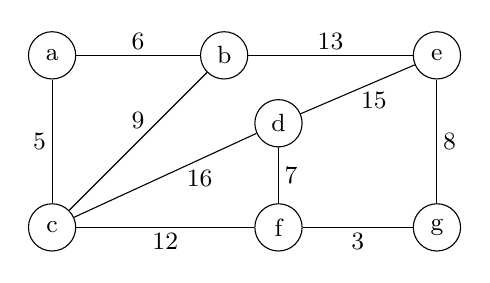
\begin{tikzpicture}[x=1.15cm,y=1.15cm,v/.style={circle,draw,inner sep=0pt,minimum size=6mm,font=\small},
  w/.style={font=\small,inner sep=2pt}]
\node[v] (a) at (0,0) {a};
\node[v] (b) at (1.9,0) {b};
\node[v] (e) at (4.25,0) {e};
\node[v] (d) at (2.5,-0.75) {d};
\node[v] (c) at (0,-1.9) {c};
\node[v] (f) at (2.5,-1.9) {f};
\node[v] (g) at (4.25,-1.9) {g};
\draw (a) -- node[w,above] {6} (b);
\draw (b) -- node[w,above] {13} (e);
\draw (a) -- node[w,left] {5} (c);
\draw (b) -- node[w,pos=0.35,left=3pt] {9} (c);
\draw (c) -- node[w,pos=0.6,below right=-1pt] {16} (d);
\draw (d) -- node[w,below right=-1pt] {15} (e);
\draw (d) -- node[w,right] {7} (f);
\draw (e) -- node[w,right] {8} (g);
\draw (c) -- node[w,below] {12} (f);
\draw (f) -- node[w,below] {3} (g);
\end{tikzpicture}
\end{center}
\item[㈡] 請定義生成樹（spanning tree）。（6 分）
\item[㈢] 請畫出此圖的最小成本生成樹（minimum cost spanning tree），以及計算最小成本。（10 分）
\end{enumerate}
\end{pastexam}

\begin{pastsoln}
\textbf{㈠} 圖有 $7$ 個頂點、$10$ 條無向邊，邊上有權重。 用 $7 \times 7$ 的矩陣，$W[u][v]$ 放邊
$(u, v)$ 的權重，沒有邊放 $\infty$，對角線放 $0$（資結書第~21.2~節）。 無向圖的矩陣對稱。
\begin{center}
\small
\begin{tabular}{c|ccccccc}
 & a & b & c & d & e & f & g \\
\hline
a & 0 & 6 & 5 & $\infty$ & $\infty$ & $\infty$ & $\infty$ \\
b & 6 & 0 & 9 & $\infty$ & 13 & $\infty$ & $\infty$ \\
c & 5 & 9 & 0 & 16 & $\infty$ & 12 & $\infty$ \\
d & $\infty$ & $\infty$ & 16 & 0 & 15 & 7 & $\infty$ \\
e & $\infty$ & 13 & $\infty$ & 15 & 0 & $\infty$ & 8 \\
f & $\infty$ & $\infty$ & 12 & 7 & $\infty$ & 0 & 3 \\
g & $\infty$ & $\infty$ & $\infty$ & $\infty$ & 8 & 3 & 0 \\
\end{tabular}
\end{center}
若只要表示「有沒有邊」，把有權重的格子換成 $1$、$\infty$ 和對角線換成 $0$ 即可；這題的圖有權重，
㈢ 要用到，所以寫權重矩陣比較完整。

\textbf{㈡} 連通無向圖 $G = (V, E)$ 的生成樹是 $G$ 的一個子圖 $T = (V, E')$，$E' \subseteq E$，滿足：
包含 $G$ 的\textbf{所有}頂點，而且 $T$ 是一棵樹，也就是連通、沒有環。 等價的說法：$T$ 用了
$G$ 的 $|V| - 1$ 條邊而且連通（或 $|V| - 1$ 條邊而且沒有環）。 生成樹是「把所有頂點連起來最少要
幾條邊」的答案：少一條就不連通，多一條就有環。 帶權重的圖裡，邊的權重和最小的生成樹叫做最小成本
生成樹（資結書第~24.1~節）。 $G$ 不連通時沒有生成樹。

\textbf{㈢} 用 Kruskal 演算法（資結書第~24.2~節）：邊依權重由小到大看，兩端已經連通（加了會成環）
就跳過，否則加入。
\begin{center}
\small
\begin{tabular}{cccl}
\toprule
權重 & 邊 & 結果 & 加入後的連通塊（只列兩點以上的） \\
\midrule
3 & f--g & 加入 & $\{f, g\}$ \\
5 & a--c & 加入 & $\{a, c\}$, $\{f, g\}$ \\
6 & a--b & 加入 & $\{a, b, c\}$, $\{f, g\}$ \\
7 & d--f & 加入 & $\{a, b, c\}$, $\{d, f, g\}$ \\
8 & e--g & 加入 & $\{a, b, c\}$, $\{d, e, f, g\}$ \\
9 & b--c & 跳過（b、c 已連通） & \\
12 & c--f & 加入 & 全部 $7$ 個頂點 \\
\bottomrule
\end{tabular}
\end{center}
加到第 $6 = 7 - 1$ 條邊就完成；剩下的 13（b--e）、15（d--e）、16（c--d）兩端都已連通，不會被選。
\begin{center}
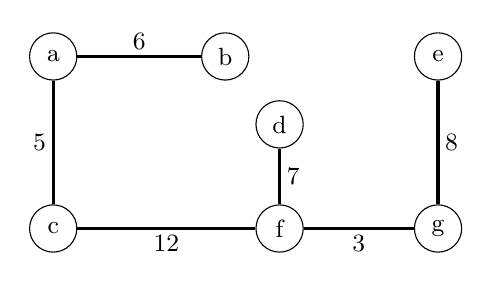
\begin{tikzpicture}[x=1.15cm,y=1.15cm,v/.style={circle,draw,inner sep=0pt,minimum size=6mm,font=\small},
  w/.style={font=\small,inner sep=2pt}]
\node[v] (a) at (0,0) {a};
\node[v] (b) at (1.9,0) {b};
\node[v] (e) at (4.25,0) {e};
\node[v] (d) at (2.5,-0.75) {d};
\node[v] (c) at (0,-1.9) {c};
\node[v] (f) at (2.5,-1.9) {f};
\node[v] (g) at (4.25,-1.9) {g};
\draw[very thick] (a) -- node[w,above] {6} (b);
\draw[very thick] (a) -- node[w,left] {5} (c);
\draw[very thick] (d) -- node[w,right] {7} (f);
\draw[very thick] (e) -- node[w,right] {8} (g);
\draw[very thick] (c) -- node[w,below] {12} (f);
\draw[very thick] (f) -- node[w,below] {3} (g);
\end{tikzpicture}
\end{center}
最小成本 $= 3 + 5 + 6 + 7 + 8 + 12 = 41$。 十條邊的權重互不相同，所以最小生成樹只有這一棵
（資結書定理~24.4）；用 Prim 演算法從任何頂點開始也會得到同樣六條邊。
\end{pastsoln}
